\documentclass[11pt]{exam}
\usepackage{array}
\usepackage{amsmath} 
\usepackage{enumerate} 
\usepackage{tcolorbox}

\usepackage{hyperref}
% See geometry.pdf to learn the layout options. There are lots.
%\geometry{letterpaper}                   % ... or a4paper or a5paper or ... 
%\geometry{landscape}                % Activate for for rotated page geometry
%\usepackage[parfill]{parskip}    % Activate to begin paragraphs with an empty line rather than an indent
%\usepackage[margin=.7in]{geometry}
\usepackage[letterpaper]{geometry}
\geometry{tmargin=0.7in,bmargin=0.85in,lmargin=0.6in,rmargin=0.6in}
\usepackage{graphicx, tikz}
\usetikzlibrary{arrows}
\usetikzlibrary{decorations.markings}
\tikzstyle arrowstyle=[scale=1]
\tikzstyle directed=[postaction={decorate,decoration={markings,
    mark=at position .65 with {\arrow[arrowstyle]{stealth}}}}]
\tikzstyle reverse directed=[postaction={decorate,decoration={markings,
    mark=at position .65 with {\arrowreversed[arrowstyle]{stealth};}}}]



\usetikzlibrary{graphs,graphs.standard} % for drawing complete graphs





\usepackage{amssymb}
\usepackage{epstopdf}
\DeclareGraphicsRule{.tif}{png}{.png}{`convert #1 `dirname #1`/`basename #1 .tif`.png}

\usepackage{pifont}% http://ctan.org/pkg/pifont
\newcommand{\cmark}{\ding{51}}%
\newcommand{\xmark}{\ding{55}}%

\addpoints

\usepackage{pgfplots} % for drawing graph

\newcommand{\ds}{\displaystyle}
\newcommand{\dx}{\text{ dx}}
\newcommand{\dz}{\text{ dx}}
\newcommand{\dy}{\text{ dy}}


\def\mycoursenumber{Math-3250}
\def\mycoursename{Combinatorics}
\def\mysemester{Spring 2019}
\def\myexamnumber{}
\def\mydate{}


\newcommand{\vect}[1]{\left\langle #1 \right \rangle}

\def\tfblank{$\underline{\phantom{xxxx}}$\quad}

\def\blank#1{\underline{\phantom{#1#1}}}


\pointsinrightmargin
\bracketedpoints 


%\printanswers

%\title{Brief Article}
%\author{Review Questions for 1st Exam}
%\date{}                                           % Activate to display a given date or no date
%\textsf{}
\begin{document}

%%%%%%%%%%%%%%%%%%%%%%
%Header / Footer
%%%%%%%%%%%%%%%%%%%

\firstpageheader{\mycoursenumber \ \mycoursename}{}{Sec 2.1 Induction Review}
\firstpageheadrule
\runningheader{\mycoursenumber \ \mycoursename}{}{Sec 2.1 Induction Review}
\runningheadrule
\firstpagefooter{}{Page \thepage\ of \numpages}{}
\runningfooter{}{Page \thepage\ of \numpages}{}
\firstpagefootrule
\runningfootrule





\begin{questions}
\question
Consider the Tower of Hanoi puzzle.


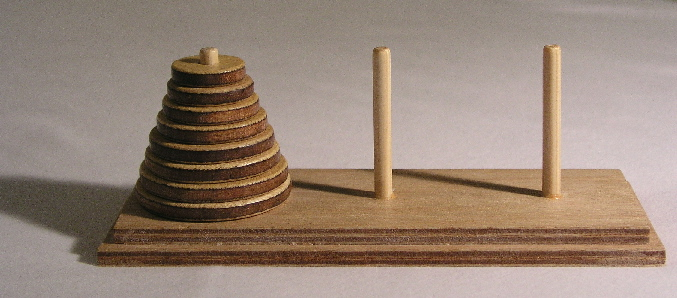
\includegraphics[width=2in]{week1d1_induction_tower_of_hanoi.jpg} 

\begin{enumerate}[i.)]
\item Is it possible to solve this puzzle in $2^n-1$ moves? Play this puzzle with your $n$ paper disks, where $n=1,2,3$, and $4$.
\item Prove (using induction) that it is possible to solve this puzzle in $2^n-1$ moves, or give a counterexample (find a number $M$ where you need more than $2^M-1$ to solve the puzzle).
\begin{solution}
See Gilbert-Vanstone `An intro to mathematical thinking', the textbook for Math 2710 UConn course, page 94.
\end{solution}
%\vfill
\end{enumerate}

%\question
%There are $N$ students in this class. I want to make sure that everyone is paired with everyone else exactly once during the semester.
%\begin{enumerate}[a.)]
%\item 
%How many times should I schedule pair activities? Write the answer as an explicit (closed-form) formula.
%\item Prove your closed-form formula using induction.
%
%\end{enumerate}
%
%\question
%To make sure everyone knows everyone, 
%please have everyone shake hands or fist-bump with everyone in the group. Then count the number of occurrences.
%\begin{enumerate}[A.)]
%\item If there are $N$ people in a large group, how many handshakes will happen if everyone shakes hands exactly once with everyone in the group? Write the answer as an explicit (closed-form) formula.
%\item Prove your closed-form formula using induction.
%\end{enumerate}

\question
On the board, please draw the complete graph on $5$ vertices 

\begin{tikzpicture}[scale=1]
  \graph { subgraph K_n [n=5,clockwise,radius=0.9cm] };
\end{tikzpicture}
 
Count the number of edges in this graph.

\begin{enumerate}[I.)]
\item How many edges are there for the complete graph on $N$ vertices? Write the answer as an explicit (closed-form) formula.
\item Prove your closed-form formula using induction.
\end{enumerate}

%\vfill\vfill\vfill
\begin{solution}
${n \choose 2}$ which is $\displaystyle \frac{n(n-1)}{2}$.
\end{solution}


\question 
The following even numbers can be written as the sum of two primes:
\begin{align*}
6 &= 3 + 3 \\
8 &= 3 + 5 \\
10 &= 3 + 7 = 5 + 5 \\
12 &= 7 + 5
\end{align*}

\begin{enumerate}[a.]
\item Write each of the even numbers $50$, $70$, and $100$ as the sum of two primes. Find as many ways as possible to write them as sums of two primes.

\item Is it possible to write every even number (larger than $2$) as the sum of two primes? 
\item Prove (using induction) that it is possible, or give a counterexample (find an even number $M>2$ which cannot be written as the sum of two primes).
\end{enumerate}

\begin{solution}
100 = 3 + 97 = 11 + 89 = 17 + 83 = 29 + 71 = 41 + 59 = 47 + 53.\\
This is the Goldbach conjecture.
\end{solution}


\end{questions}

\end{document}  
